%
% File emnlp2016.tex
%

\documentclass[11pt,letterpaper]{article}

\usepackage{emnlp2016}
\usepackage{times}
\usepackage{latexsym}

% reference main submission for equations, etc.
\usepackage{xr}
\externaldocument{emnlp2016}
\setcounter{equation}{5}
\setcounter{table}{5}
\setcounter{figure}{5}% TODO: make sure these are accurate

% \RequirePackage[l2tabu, orthodox]{nag}
% \documentclass{article}

% % FONTS
\usepackage[T1]{fontenc}

% Replace default Latin Modern typewriter with its proportional counterpart
% http://www.tug.dk/FontCatalogue/lmoderntypewriterprop/
\renewcommand*\ttdefault{lmvtt}

%\usepackage[bitstream-charter]{mathdesign} % not needed for mtpro
\usepackage{amsmath}
\usepackage[subscriptcorrection,
            amssymbols,
            mtpbb,
            mtpcal,
            nofontinfo  % suppresses all warnings
           ]{mtpro2} %TODO: put htis back in and take out mathdesign
\usepackage{scalefnt,letltxmacro}
\LetLtxMacro{\oldtextsc}{\textsc}
\renewcommand{\textsc}[1]{\oldtextsc{\scalefont{1.10}#1}}
\usepackage[scaled=0.92]{PTSans}


% % COLOR
\usepackage[usenames,dvipsnames]{xcolor}
\definecolor{Green}{HTML}{156946}

% % SPACING and TEXT
\usepackage[final,expansion=alltext]{microtype}
\usepackage[english]{babel}
\usepackage{afterpage}
\usepackage{framed}


% define a paragraph header function
\DeclareRobustCommand{\parhead}[1]{\textbf{#1}~}

% % EDITING
% paragraph helper
\DeclareRobustCommand{\PP}{\textcolor{Plum}{\P} }

% % COUNTERS
\usepackage{enumitem}
\renewcommand{\labelenumi}{\color{black!67}{\arabic{enumi}.}}
\renewcommand{\labelenumii}{{\color{black!67}(\alph{enumii})}}
\renewcommand{\labelitemi}{{\color{black!67}\tiny$\blacksquare$}}
\renewcommand{\labelitemii}{{\color{black!67}\textbullet}}
\renewcommand{\labelitemiii}{{\color{black!67}\scriptsize$\blacktriangleright$}}

% FIGURES
\usepackage{graphicx}

% TABLES
\usepackage{booktabs}

% ALGORITHMS
\usepackage[algoruled]{algorithm2e}
\usepackage{listings}
\usepackage{fancyvrb}
\fvset{fontsize=\normalsize}

% % HYPERREF
\usepackage[colorlinks,linktoc=all]{hyperref} %TODO: rm draft
\usepackage[all]{hypcap}
\hypersetup{citecolor=Green}
\hypersetup{linkcolor=Green}
\hypersetup{urlcolor=Green}

% % CLEVEREF must come after HYPERREF
\usepackage[nameinlink]{cleveref}

% BIBLIOGRPHY: get rid of reference labels
\makeatletter
	\renewcommand\@biblabel[1]{}
\makeatother

% ACRONYMS
\usepackage[acronym,smallcaps,nowarn]{glossaries}
% \makeglossaries

% % COLOR DEFINITIONS
\newcommand{\green}[1]{\textcolor{Green}{#1}}


% LISTINGS DEFINTIONS
\lstdefinestyle{mystyle}{
    commentstyle=\color{Green},
    keywordstyle=\color{Green},
    numberstyle=\tiny\color{black!60},
    stringstyle=\color{Green},
    basicstyle=\ttfamily,
    breakatwhitespace=false,
    breaklines=true,
    captionpos=b,
    keepspaces=true,
    numbers=left,
    numbersep=5pt,
    showspaces=false,
    showstringspaces=false,
    showtabs=false,
    tabsize=2
}
\lstset{style=mystyle}

% ALGORITHMS
\usepackage[algoruled]{algorithm2e}

% FRAMES
\usepackage[linewidth=1pt]{mdframed}
\DeclareRobustCommand{\mb}[1]{\ensuremath{\boldsymbol{\mathbf{#1}}}}

\DeclareMathOperator*{\argmax}{arg\,max}
\DeclareMathOperator*{\argmin}{arg\,min}

\DeclareRobustCommand{\KL}[2]{\ensuremath{\textrm{KL}\left(#1\;\|\;#2\right)}}

\newcommand{\mbx}{\mathbold{x}}
\newcommand{\mbX}{\mbf{X}}

\newcommand{\mbz}{\mathbold{z}}

\newcommand{\mbI}{\mbf{I}}

\newcommand{\mbZ}{\mbf{Z}}
\newcommand{\mbL}{\mbf{L}}

\newcommand{\mbtheta}{\mathbold{\theta}}
\newcommand{\mbTheta}{\mathbold{\Theta}}
\newcommand{\mbomega}{\mathbold{\omega}}
\newcommand{\mbOmega}{\mathbold{\Omega}}
\newcommand{\mbsigma}{\mathbold{\sigma}}
\newcommand{\mbSigma}{\mathbold{\Sigma}}

\newcommand{\mblambda}{\mathbold{\lambda}}
\newcommand{\mbgamma}{\mathbold{\gamma}}
\newcommand{\mbzeta}{\mathbold{\zeta}}
\newcommand{\mbeta}{\mathbold{\eta}}
\newcommand{\mbbeta}{\mathbold{\beta}}
\newcommand{\mbphi}{\mathbold{\phi}}
\newcommand{\mbmu}{\mathbold{\mu}}
\newcommand{\mbrho}{\mathbold{\rho}}

\newcommand\dif{\mathop{}\!\mathrm{d}}
\newcommand{\diag}{\textrm{diag}}
\newcommand{\supp}{\textrm{supp}}

\newcommand{\E}{\mathbb{E}}
\newcommand{\Var}{\mathbb{V}\textrm{ar}}

\newcommand{\bbN}{\mathbb{N}}
\newcommand{\bbZ}{\mathbb{Z}}
\newcommand{\bbR}{\mathbb{R}}
\newcommand{\bbS}{\mathbb{S}}

\newcommand{\cL}{\mathcal{L}}

\newcommand{\cN}{\mathcal{N}}
\newcommand{\Gam}{\textrm{Gam}}
\newcommand{\InvGam}{\textrm{InvGam}}

\newcommand{\g}{~\vert~}
\newacronym{KL}{kl}{Kullback-Leibler}
\newacronym{ELBO}{elbo}{\emph{evidence lower bound}}
\newacronym{POPELBO}{pop-elbo}{\emph{population evidence lower bound}}

\newacronym{SVI}{svi}{stochastic variational inference}
\newacronym{BUMPVI}{bump-vi}{bumping variational inference}

\newacronym{GMM}{gmm}{Gaussian mixture model}
\newacronym{LDA}{lda}{latent Dirichlet allocation}

\newacronym{SUTVA}{sutva}{stable unit treatment value assumption}


% Uncomment this line for the final submission:
%\emnlpfinalcopy

%  Enter the EMNLP Paper ID here:
\def\emnlppaperid{***} % TODO

% To expand the titlebox for more authors, uncomment
% below and set accordingly.
% \addtolength\titlebox{.5in}    

\title{Detecting and Characterizing Events: Appendices}

% Author information can be set in various styles:
% For several authors from the same institution:
% \author{Author 1 \and ... \and Author n \\
%         Address line \\ ... \\ Address line}
% if the names do not fit well on one line use
%         Author 1 \\ {\bf Author 2} \\ ... \\ {\bf Author n} \\
% For authors from different institutions:
% \author{Author 1 \\ Address line \\  ... \\ Address line
%         \And  ... \And
%         Author n \\ Address line \\ ... \\ Address line}
% To start a seperate ``row'' of authors use \AND, as in
% \author{Author 1 \\ Address line \\  ... \\ Address line
%         \AND
%         Author 2 \\ Address line \\ ... \\ Address line \And
%         Author 3 \\ Address line \\ ... \\ Address line}
% If the title and author information does not fit in the area allocated,
% place \setlength\titlebox{<new height>} right after
% at the top, where <new height> can be something larger than 2.25in
\author{
Allison J.B. Chaney\\
    Princeton University\\
	\href{mailto:achaney@cs.princeton.edu}{\nolinkurl{achaney@cs.princeton.edu}}
\And
Hanna Wallach\\
    Microsoft Research\\
    \href{mailto:wallach@microsoft.com}{\nolinkurl{wallach@microsoft.com}}
\AND
David M. Blei\\
    Columbia University\\
    \href{mailto:david.blei@columbia.edu}{\nolinkurl{david.blei@columbia.edu}}
\And
Matthew Connelly\\
    Columbia University\\
    \href{mailto:mjc96@columbia.edu}{\nolinkurl{mjc96@columbia.edu}}
}

\date{}

\begin{document}

\maketitle

\appendix
\section{Inference}
\label{sec:inference}
%!TEX root = supplemental.tex

In this appendix, we describe the details of the inference algorithm for Capsule.

Conditional on a collection of observed documents, our goal is to estimate the posterior values of the hidden parameters, according to the Capsule model.   Recall that our data is observed as word counts $w_{d,v}$ for document $d$ and vocabulary term $v$, with corresponding author and time interval information for each document---$a_d$ and $i_d$, respectively.
The latent parameters of the model include general topics $\beta$, entity topics $\eta$, and interval topics $\gamma$, as well as document-specific strengths in each of these spaces: document relevancy to general topics $\theta$, entity topics $\zeta$, and interval topics $\epsilon$.  The latent parameters also include entity concerns with general topics $\phi$ and with entity-specific topics $\xi$, and overall event strength $\psi$.  See \Cref{fig:generative-model} for the full generative model.

As for many Bayesian models, the exact posterior for Capsule is not tractable to compute; we must instead approximate it.  Thus, we develop an approximate inference algorithm for Capsule based on variational methods~\cite{Jordan:1999,Wainwright:2008}.

Variational inference approaches the problem of posterior inference by minimizing the KL divergence from an approximating distribution $q$ to the true posterior $p$.
This is equivalent to maximizing the ELBO,
\begin{multline}
	\mathcal{L}(q)  = \E_{q}\bigl[\log p(w, \psi, \gamma, \phi, \beta, \xi, \eta, \theta, \epsilon, \zeta) 
	-\\ \log q(\psi, \gamma, \phi, \beta, \xi, \eta, \theta, \epsilon, \zeta)\bigr].
	\label{eq:cables:elbo}
\end{multline}


We define the approximating distribution $q$ using the mean field assumption:
\begin{multline}
	q(\psi, \gamma, \phi, \beta, \xi, \eta, \theta, \epsilon, \zeta) = \\
	 	\prod_{d=1}^D \left[q(\zeta_d \g \lambda_d)
				\prod_{k=1}^K q(\theta_{d,k} \g \lambda^\theta_{d,k})
				\prod_{t=1}^T q(\epsilon_{d,t} \g \lambda^\epsilon_{d,t})
			\right] \\
		\prod_{t=1}^T \left[ q(\gamma_{t} \g \lambda^\gamma_t) q(\psi_t \g \lambda^\psi_t) \right] \\
		\prod_{n=1}^N \left[ q(\xi_{n} \g \lambda^\xi_{n})~q(\eta_n \g \lambda^{\eta}_{n}) \right] \\
		\prod_{k=1}^K \left[ q(\beta_{k} \g \lambda^\beta_k) \prod_{n=1}^N q(\phi_{n,k} \g \lambda^\phi_{n,k}) \right]
	\label{eq:q}
\end{multline}

The variational distributions for the topics $q(\gamma)$, $q(\beta)$ and $q(\eta)$ are all Dirichlet-distributed with free variational parameters $\lambda^\gamma$, $\lambda^\beta$, and $\lambda^\eta$ respectively.  Similarly, the variational distributions $q(\psi)$, $q(\phi)$, $q(\xi)$, $q(\theta)$, $q(\epsilon)$, and $q(\zeta)$ are all gamma-distributed with corresponding free variational parameters $\lambda^\psi$, $\lambda^\phi$, $\lambda^\xi$, $\lambda^\theta$, $\lambda^\epsilon$ and $\lambda^\zeta$.  For these gamma-distributed variables, each free parameter $\lambda$ has two components: shape $s$ and rate $r$.

The expectations under $q$, which are needed to maximize the ELBO, have closed form analytic updates--we update each parameter in turn, following standard coordinate ascent variational inference techniques, as the Capsule model is specified with the required conjugate relationships that make this approach possible~\cite{Ghahramani:2001}.


To obtain simple updates, we first rely on auxiliary latent variables $z$. These variables, when marginalized out, leave the original model intact. The Poisson distribution has an additive property; specifically if $w \sim \mbox{Poisson}(a+b)$, then $w = z_1 + z_2$, where $z_1 \sim \mbox{Poisson}(z_1)$ and $z_2 \sim \mbox{Poisson}(z_2)$.  We apply this property to the word count rate in \Cref{eq:poisrate} and define Poisson variables for each component of the word count:
\[ z^\mathcal{K}_{d,v,k} \sim \mbox{Poisson}(\theta_{d,k}\beta_{k,v}), \]
\[ z^\mathcal{E}_{d,v} \sim \mbox{Poisson}(\zeta_{d}\eta_{a_d,v}), \]
\[ z^\mathcal{T}_{d,v,t} \sim \mbox{Poisson}\left(f(i_d, t) \epsilon_{d,t} \gamma_{t,v}\right). \]
The $\mathcal{K}$, $\mathcal{E}$, and $\mathcal{T}$ superscripts indicate the contributions from general, entity, and event topics, respectively.  Given these variables, the total word count is deterministic:
\[ w_{d,v} = \sum_{k=1}^K z^\mathcal{K}_{d,v,k} + z^\mathcal{E}_{d} + \sum_{t=1}^T z^\mathcal{T}_{d,v,t}. \]

Coordinate-ascent variational inference is derived from complete conditionals, i.e., the conditional distributions of each variable given the other variables and observations. These conditionals define both the form of each variational factor and their updates. The following are the complete conditional for each of the gamma- and Dirchlet-distributed latent parameters.  The notation $D(n)$ is used for the set of documents sent by entity $n$; $D(t)$ is the set of documents sent impacted by events at time $t$ (e.g., all documents after the event in the case of exponential decay).
\begin{multline}
\gamma_t \g \mathbf{W}, \psi, \phi, \xi, \beta, \eta, \theta, \epsilon, \zeta, z \sim \\
	\mbox{Dirichlet}_V\left(\alpha_\gamma + \sum_{d=1}^D \langle
		z^\mathcal{T}_{d,1,t}, \cdots, z^\mathcal{T}_{d,V,t}\rangle
	\right)
\label{eq:pi}
\end{multline}
\begin{multline}
\eta_n \g \mathbf{W}, \psi, \phi, \xi, \beta, \gamma, \theta, \epsilon, \zeta, z \sim \\
	\mbox{Dirichlet}_V\left(\alpha_\eta + \sum_{d\in D(n)} \langle
		z^\mathcal{E}_{d,v}, \cdots, z^\mathcal{E}_{d,v}\rangle
	\right)
\label{eq:eta}
\end{multline}
\begin{multline}
\beta_k \g \mathbf{W}, \psi, \phi, \xi, \gamma, \eta, \theta, \epsilon, \zeta, z \sim \\
	\mbox{Dirichlet}_V\left(\alpha_\beta + \sum_{d=1}^D \langle
		z^\mathcal{K}_{d,1,k}, \cdots, z^\mathcal{K}_{d,V,k}\rangle
	\right)
\label{eq:beta}
\end{multline}
\begin{multline}
\psi_t \g \mathbf{W}, \phi, \xi, \beta, \gamma, \eta, \theta, \epsilon, \zeta, z \sim \\
	\mbox{Gamma}\left(
		s_\psi + |D(t)| s_\epsilon,
		r_\psi + \sum_{d\in D(t)} \epsilon_{d,t}
	\right)
\label{eq:psi}
\end{multline}
\begin{multline}
\xi_n \g \mathbf{W}, \psi, \phi, \beta, \gamma, \eta, \theta, \epsilon, \zeta, z \sim \\
	\mbox{Gamma}\left(
		s_\xi + |D(n)| s_\zeta,
		r_\xi + \sum_{d\in D(n)} \zeta_{d}
	\right)
\label{eq:xi}
\end{multline}
\begin{multline}
\phi_{n,k} \g \mathbf{W}, \psi, \xi, \beta, \gamma, \eta, \theta, \epsilon, \zeta, z \sim \\
	\mbox{Gamma}\left(
		s_\phi + |D(n)| s_\theta,
		r_\phi + \sum_{d\in D(n)} \theta_{d,k}
	\right)
\label{eq:phi}
\end{multline}
\begin{multline}
\theta_{d,k} \g \mathbf{W}, \psi, \phi, \xi, \beta, \gamma, \eta, \epsilon, \zeta, z \sim \\
	\mbox{Gamma}\left(
		s_\theta + \sum_{v=1}^V z^\mathcal{K}_{d,v,k},
		\phi_{a_d,k} + \sum_{v=1}^V \beta_{k,v}
	\right)
\label{eq:theta}
\end{multline}
\begin{multline}
\epsilon_{d,t} \g \mathbf{W}, \psi, \phi, \xi, \beta, \gamma, \eta, \theta, \zeta, z \sim \\
	\mbox{Gamma}\left(
		s_\epsilon + \sum_{v=1}^V z^\mathcal{T}_{d,v,t},
		\psi_t + f(i_d, t) \sum_{v=1}^V \gamma_{t,v}
	\right)
\label{eq:epsilon}
\end{multline}
\begin{multline}
\zeta_{d} \g \mathbf{W}, \psi, \phi, \xi, \beta, \gamma, \eta, \theta, \epsilon, z \sim \\
	\mbox{Gamma}\left(
		s_\zeta + \sum_{v=1}^V z^\mathcal{E}_{d,v},
		\xi_{a_d} + \sum_{v=1}^V \eta_{a_d,v}
	\right)
\label{eq:zeta}
\end{multline}

The complete conditional for the auxiliary variables has the form
\[z_{d,v} \g \psi, \phi, \xi, \beta, \gamma, \eta, \theta, \epsilon, \zeta \sim \mbox{Mult}(w_{d,v}, \omega_{d,v}),\] where
\begin{multline}
\omega_{d,v} \propto \langle 
\theta_{d,1} \beta_{1,v}, \cdots, \theta_{d,K} \beta_{K,v}, \zeta_d \eta_{a_d,v}, \\
f(i_d, 1) \epsilon_{d,1} \gamma_{1,v}, \cdots, f(i_d, T) \epsilon_{d,T} \gamma_{T,v}\rangle.
\label{eq:omega}
\end{multline}
Intuitively, these variables allocate the data to one of the entity concerns or events, and thus can be used to explore the data.

Given these conditionals, the algorithm sets each parameter to the expected conditional parameter under the variational distribution. The mean field assumption guarantees that this expectation will not involve the parameter being updated.  \Cref{alg:capsule} shows our variational inference algorithm.

This algorithm uses the notation $\mathbold{\lambda}$ to refer to the set of variational parameters,
\[\mathbold{\lambda} = \{\lambda^\gamma, \lambda^\eta, \lambda^\beta, \lambda^\psi, \lambda^\zeta, \lambda^\phi, \lambda^\theta, \lambda^\epsilon, \lambda^\xi\}.\] The notation $V(d)$ is the set of vocabulary indices for the collection of words in document $d$.  We could also iterate over all $V$, but as zero word counts give $\E[z_{d,v}] = 0~\forall v \not\in V(d)$, the two are equivalent.

%TODO: check for consistent indexing of variables (e.g., beta_{v,k} vs beta_{k,v})


\begin{algorithm}[p]
\small
\DontPrintSemicolon
\KwIn{word counts $w$}
%($\psi$, $\gamma$, $\xi$, $\eta$, $\phi$, $\beta$, $\theta$, $\zeta$, $\epsilon$)
\KwOut{approximate posterior of latent parameters in terms of variational parameters $\mathbold{\lambda}$}
\textbf{Initialize} $\E[\beta]$ to slightly random around uniform \;
\textbf{Initialize} $\E[\mbox{all other parameters}]$ to uniform \;
\For {iteration $m=1:M$}{
	\textbf{set} all $\mathbold{\lambda}$ to respective priors, excluding $\lambda^{\theta,rate}$, $\lambda^{\zeta,rate}$, and $\lambda^{\epsilon,rate}$, which are set to 0 \;
	\textbf{update} $\lambda^{\theta,rate} \pluseq \sum_V \E[\beta_v]$ \;
	\For {each document $d=1:D$}{
		\For {each term $v\in V(d)$\footnotemark}{
			\textbf{set} $(K+T+1)$-vector $\omega_{d,v}$ as shown in \cref{eq:omega}, using $\E$ of parameters\;
			\textbf{set} $(K+T)$-vector $\E[z_{d,v}] = w_{d,v} * \omega_{d,v}$ \;
			\textbf{update} $\lambda^{\theta,shape}_d \pluseq \E[z^\mathcal{K}_{d,v}]$ [\cref{eq:theta}]\;
			\textbf{update} $\lambda^{\epsilon,shape}_d \pluseq \E[z^\mathcal{K}_{d,v}]$ [\cref{eq:epsilon}]\;
			\textbf{update} $\lambda^{\zeta,shape}_d \pluseq \E[z^\mathcal{E}_{d,v}]$ [\cref{eq:zeta}]\;

			\textbf{update} $\lambda^{\beta}_v \pluseq \E[z^\mathcal{K}_{d,v}]$ [\cref{eq:beta}]\;
			\textbf{update} $\lambda^{\gamma}_v \pluseq \E[z^\mathcal{T}_{d,v}]$ [\cref{eq:pi}]\;
			\textbf{update} $\lambda^{\eta}_v \pluseq \E[z^\mathcal{E}_{d,v}]$ [\cref{eq:eta}]\;
		}
		\textbf{set} $\lambda^{\theta,rate}_{d} = \E[\phi_{a_d}] +\sum_v \E[\beta]$ [\cref{eq:theta}]\;
		\textbf{set} $\lambda^{\epsilon,rate}_{d} = \E[\psi] + f\sum_v \E[\gamma]$ [\cref{eq:epsilon}]\;
		\textbf{set} $\lambda^{\zeta,rate}_{d} = \E[\xi_{a_d}] + \sum_v\E[\eta]$ [\cref{eq:zeta}]\;
		
		\textbf{set} $\E[\theta_d] = \lambda^{\theta,shape}_d / \lambda^{\theta,rate}_d$ \;
		\textbf{set} $\E[\epsilon_d] = \lambda^{\epsilon,shape}_d / \lambda^{\epsilon,rate}_d$ \;
		\textbf{set} $\E[\zeta_d] = \lambda^{\zeta,shape}_d / \lambda^{\zeta,rate}_d$ \;
		
		\textbf{update} $\lambda^{\phi,shape}_{a_d} \pluseq s_\theta$ [\cref{eq:phi}] \;
		\textbf{update} $\lambda^{\psi,shape}_{t} \pluseq s_\epsilon \forall t : f(i_d, t) \neq 0$ [\cref{eq:psi}] \;
		\textbf{update} $\lambda^{\xi,shape}_{a_d} \pluseq s_\eta$ [\cref{eq:xi}] \;
		\textbf{update} $\lambda^{\phi,rate}_{a_d} \pluseq \theta_d$ [\cref{eq:phi}] \;
		\textbf{update} $\lambda^{\psi,rate} \pluseq \epsilon_d$ [\cref{eq:psi}] \;
		\textbf{update} $\lambda^{\xi,rate}_{a_d} \pluseq \zeta_d$ [\cref{eq:xi}] \;

	}

	\textbf{set} $\E[\phi] = \lambda^{\phi,shape} / \lambda^{\phi,rate}$ \;
	\textbf{set} $\E[\beta_k] = \lambda^{\beta_{k,v}} / \sum_v \lambda^{\beta_k} \forall k$ \;
	\textbf{set} $\E[\xi] = \lambda^{\xi,shape} / \lambda^{\xi,rate}$ \;
	\textbf{set} $\E[\eta_n] = \lambda^{\eta_{n,v}} / \sum_v \lambda^{\eta_n} \forall n$ \;
	\textbf{set} $\E[\psi] = \lambda^{\psi,shape} / \lambda^{\psi,rate}$ \;
	\textbf{set} $\E[\gamma_t] = \lambda^{\gamma_{t,v}} / \sum_v \lambda^{\gamma_t} \forall t$ \;
}
\Return{$\lambda$} \;
\caption{Variational Inference for Capsule}
\label{alg:capsule}
\end{algorithm}

This algorithm produces a fitted variational distribution which can then be used as a proxy for the true posterior, allowing us to explore a collection of documents with Capsule.  Source code is available at \url{https://github.com/ajbc/capsule}.




\section{Additional Results}
\label{sec:additional_results}
%!TEX root = supplemental.tex

In this appendix, we present non-crucial experimental results for Capsule.

%%%%%%%%%%%%%%%%%%%
% Appendix~\ref{sec:additional_results} contains additional examples of events discovered by Capsule, and more examples of general and entity-specific topics.

\parhead{Events detected by Capsule.}
In addition to the real-world events discussed in \Cref{sec:eval}, many other events were detected by Capsule.  For example, in 1973, the U.S. presented all nations with samples of rock obtained from the moon on the Apollo 17 mission.  Top cables under $\epsilon$ for this week include messages about receiving the sample shipments at the various embassies, such as a message sent by the Cairo embassy on July 2, 1973:
\begin{shaded*} \tt{Lunar sample recieved June 30.  Will advise Department of our plans for presentation as soon as they are firm.}
\end{shaded*}
\noindent and a similar message from the Kuala Lumpur Embassy the same day:
\begin{shaded*} \tt{Lunar sample and accompanying materials unreceived. Advise shipping data.}
\end{shaded*}
\noindent We also observe a cable sent by New Delhi the following day:
\begin{shaded*} \tt{1. As Department aware, lunar sample for India was presented by Apollo 17 austronauts to Lok Sabha (Lower House of Parliment) Speaker G.S.~Dhillon on Jun 19.
Captain Cernan's remarks on that occasion on which he was escorted by the Charge',
were similar to those suggested Ref B.}

\tt{2. Embassy has received lunar sample for Bhutan (Ref A) which will be presented to Bhutanese on some propitious future date.
In making presentation, remarks suggested Ref B will be drawn upon as appropriate.}
\end{shaded*}


Another peak in \Cref{fig:cables_events} occurs the week of April 17, 1978 surrounding a UN special session on disarmament; the top three words under event its description $\pi$ are \emph{SSOD} (acronym for ``special session on disarmament'', \emph{disarmament}, and \emph{ICS} (likely an acronym for ``incident command system''); \Cref{tab:ssod} shows the top cables for this time interval, sorted by event relevancy $\epsilon$.  Most of these cables concern attendance, such as the first cable, which is from Bangkok:
\begin{shaded*} \tt{
Thai Ministry of Foreign Affairs official in International Organizations Department told EmbOff Apr 19 that his Dept had recommended that Foriegn Minister Uppadit attend SSOD. 
Uppadit, however, had just arrived back from trip to Asean
countries and had not yet considered composition of delegation.
MFA official expected the Foreign Minister would not decided
on his attendance until early May. Will advise.}
\end{shaded*}

\begin{table*}[tb]
\small
\centering
\begin{tabular}{cccl}
\toprule
$\epsilon$ & date & entity & subject \\
\midrule
0.084 & 1978-04-19 & Bangkok & UN Special Session on Disarmament: high level participation: Thailand \\
0.074 & 1978-04-19 & Valletta & UN Special Session on Disarmament, May 23 - June 28: high level  participation \\
0.073 & 1978-04-20 & Bern & UN Special Session on Disarmament, May 23-June 28: high- level  participation \\
0.073 & 1978-04-23 & State & High level attendance at Special Session on Disarmament (SSOD) \\
0.073 & 1978-04-21 & Lagos & UN Special Session on Disarmament, May 23-June 28: high level  participation \\
0.069 & 1978-04-19 & Madrid & UN Special Session on Disarmament May 23 - June 28: high-level  participation \\
0.067 & 1978-04-19 & Seoul & UN Special Session on Disarmament \\
0.067 & 1978-04-19 & Tehran & Iranian participation at SSOD May 23-June 28 \\
0.065 & 1978-04-19 & Niamey & UN Special Session on Disarmament, May 23-June 26 high level participation \\
0.061 & 1978-04-19 & Berlin & UN Special Session on Disarmament, May 23 - June 28; high-level participation \\
0.061 & 1978-04-18 & Sofia & official-informal \\
0.060 & 1978-04-19 & Abidjan & UN Special Session on Disarmament: Ivorian participation \\
0.056 & 1978-04-19 & Athens & UN Special Session on Disarmament, May 23-June 28: high level participation \\
0.054 & 1978-04-20 & State & SSOD: security assurances for non-nuclear states \\
0.053 & 1978-04-19 & Kuwait & UN Special Session on Disarmament (SSOD), May 23-June 28: high level ... \\%icipation \\
0.051 & 1978-04-19 & Vienna & UN Special Session on Disarmament, May 23-June 28: high level part... \\%participation from Austria \\
0.050 & 1978-04-20 & Bogota & Meeting delegations: UN Special Session on Disarmament \\
\bottomrule
\end{tabular}
\label{tab:ssod}
\caption{Top documents for the time interval of week April 17, 1978, in preparation for the a UN Special Session on Disarmament.}
\end{table*}

Unfortunately, many interesting cables are withdrawn, meaning the main body of the message is unavailable.  An example of this is the cable sent on April 20, 1978 from the State Department to London with the subject \emph{SSOD: security assurances for non-nuclear states.}  The following description is provided by NARA for withdrawn cables such as these:
\begin{shaded*}
\emph{The Department of State created withdrawal cards for telegrams exempt from disclosure for reasons of national security, privacy, and other statutory concerns. The agency's withdrawal cards serve as placeholders for the records exempt from disclosure. NARA created withdrawal cards for an additional set of telegrams that require review under the Freedom of Information Act. The data elements potentially available for each withdrawal card include: concepts; date; document number; from; subject; traffic analysis by geography and subject; to; and microfilm roll number.}
\end{shaded*}

\begin{table*}[tb]
\small
\centering
\begin{tabular}{cccl}
\toprule
$\epsilon$ & date & entity & subject \\
\midrule
0.088 & 1978-01-05 & Sarasin, Ronald A & Return of the crown of St Stephen to Hungary \\
0.088 & 1978-01-05 & Cotter, William R & Return of the crown of St Stephen to Hungary \\
0.080 & 1978-01-05 & Cranston, Alan & Return of crown of St Stephen to Hungary \\
0.078 & 1978-01-06 & Schweiker, Richard S & Return of crown of St Stephen to Hungary \\
0.076 &  1978-01-06 & Church, Frank & Return of crown of Stepeht to Hungary \\
0.076 &  1978-01-05 & Wright, Jim & Return of crown of St Stephen to Hungary \\
0.076 &  1978-01-05 & Wright, Jim & Against return of crown of St Stephen to Hungary \\
0.068 &  1978-01-03 & Tarnoff, Peter & Return of the crown of St Stephen to Hungary \\
0.066 & 1978-01-03 & Tarnoff, Peter & Return of crown of St Stephen to Hungary \\
0.056 &  1978-01-03 & Duncan, John J & Info on the crown of St Stephen of Hungary \\
0.053 &  1978-01-06 & Church, Frank & Return of crown of St Stephen to Hungarian govt \\
0.052 &  1978-01-06 & Nelson, Gaylord & Cost of Emperor Bokassa's coronation in Central African Empire \\
0.051 &  1978-01-03 & Beckel, Robert G & return of crown of St Stephen to Hungary \\
0.049 &  1978-01-05 & Cranston, Alan & Concern regarding the crown of St Stephen of Hungary \\
0.046 &  1978-01-03 & Chiles, Lawton & Against returning crown of St Stephen to Hungarian government \\
0.046 &  1978-01-05 & Secretary Paris & The crown: Mrs. Vance's schedule \\
0.043 &  1978-01-05 & Beckel, Robert G & RE constituents concern over return of crown of St. Stephen \\
\bottomrule
\end{tabular}
\label{tab:crown}
\caption{Top documents for the time interval of week of January 2, 1978, when Pres. Carter decided to return teh crown of St. Stephen to Hungary.}
\end{table*}

The return of the crown of St.~Stephen to Hungary was a contentious event, with many individuals sending in their opinions on it; \Cref{tab:crown} shows top cables for this event.

In early October of 1977, the International Whaling commission (IWC) banned killing bowhead whales. Capsule detects this surge in discussion and the top cables recovered by Capsule indicate that the U.S. State department objected to this ban,\footnote{Their objections were based on Alaskan Natives rely on these whales for sustenance.} but that many individuals disagreed, resulting in the majority of the top cables having subjects along the lines of \emph{Requests State Dept not file objection to zero quota for bowhead whales}.

Similar to the sequence of Sinai events, another sequence of events occurs surrounding opium production; in March 1974, Capsule detects that Turkey plans to lift a ban on growing opium poppy.  Two months later, the model detects another event when the U.S. makes a policy statement on the domestic production of opium poppy.  For the first event, the top three cables for this interval have subjects \emph{Turkey to resume cultivation of the opium poppy}, \emph{Cultivation of opium poppy in Turkey}, and \emph{Ban on opium cultivation in Turkey}. Another cable further down the list has the subject, \emph{US funds to Turkey to halt opium production}.  On March 12, 1975, the London embassy reports the the State Department:
\begin{shaded*}
\tt{1.  Pursuant to RefTel, we spoke to W.~N.~Hillier-Fry, 
head of Middle East and Mediterranean Department
of Overseas Development Administration, who will
head UK delegation to meeting of OECD consortium for
Turkey.  Hillier-Fry said that, as in last meeting,
he can support USG initiatives with regard to Turkish
opium production, but he emphasized that he will have
to take a very cautious approach and will pick his
words carefully.  He added that he will be in touch
with USG representatives at the meeting.}

\tt{2.  As FCO department head
in separate conversation March 11, UK representative
will have to be careful in whatever he says not to
imply any increase in British aid to Turkey, given
straitened financial circumstances of hmg at present.
Goodison also confirmed letter from him has gone to
British ambassador in Ankara along lines indicated
London's 2980.}
\end{shaded*}
\noindent Two days later, Kissinger sends a message to Ankara with the subject \emph{Opium ban: attitudes within GOT}:
\begin{shaded*}
\tt{In conversation with Sisco reported RefTel Esenbel referred
to division within got on handling of opium problems.  At
one point he identified Orhan Eyuboglu as leader of hard
liners who wished immediate resumption of poppy cultivation.  
By implication he identified Fonmin Gunes and
himself as members of those seeking cooperate with united
states, e.g. Gunes ``very pleased'' with decision not to
plant in April.}
\end{shaded*}
Eight weeks later, we see the second event with many messages on individuals writing on the subject of the \emph{US policy statement on domestic production of opium poppy}.  Again, Capsule cannot capture every aspect of larger sequences of events, but it can provide insight into key moments, as it does here.

\parhead{Topics Found by Capsule.}
\Cref{tab:generaltopics} shows a selection of general topics, including those shown in Tables~\ref{tab:3topics} and~\ref{tab:topics}.


\begin{table}
\centering
\small
\begin{tabular}{c}
\toprule
top terms \\
\midrule
plan, visit, arrival, itinerary, visitor \\
outlook, review, hire, personnel, invite, prepare \\
arrest, incident, security, family, guard, death, jail \\
locate, home, son, death, please, contact, father \\
request, refugee, response, service, sale, asylum \\
market, report, commercial, food, import, commerce \\
fear, leadership, back, arm, role, threaten \\
hotel, travel, reservation, visit, arrange, schedule \\
exchange, student, rate, assume, program, cultural \\
copy, publication, panama, brochure, material, order \\
registry, pouch, number, invoice, item, classify \\
extension, provision, decide, case, decision, effect \\
right, cause, history, solution, improve, relation \\
nation, peace, soviet, crisis, strengthen, victory \\
israel, israeli, middle, concern, charge, negotiation \\
fund, management, project, overseas, committee \\
large, industry, sell, sale, supplier, limit, firm \\
concern, right, belief, point, fact, allege, explain \\
support, election, success, war, leader, demonstrate \\
case, visa, arrive, eta, consul, embassy, travel, reftel \\
science, advisory, concern, study, request, follow \\
\bottomrule
\end{tabular}
\label{tab:generaltopics}
\caption{Top vocabulary terms for a selection of general topics, one per row, according to topic distributions $\beta_k$.}
\end{table}

\Cref{tab:enttopics} shows a selection of entity topics, including those shown in Tables~\ref{tab:entities} and~\ref{tab:topics}.

\begin{table*}
\centering
\small
\begin{tabular}{cc}
\toprule
entity & top terms \\
\midrule
Algiers & algerian, algeria, say, one, embassy, do \\
Amman & jordanian, visit, make, say, time, do, meet \\
Bangkok & bangkok, thailand, thai, refugee, follow \\
Barcelona & spain, spanish, lane, repatriation \\ 
Beirut & beirut, lebanon, lebanese, say, report \\
Brussels & belgian, brussels, belgium, meet, embassy \\
Budapest & hungarian, embassy, hungary, visit, mudd \\
Cape Town & cape, town, africa, say, african, make \\
Caracas & venezuelan, venezuela, caracas, embassy \\ 
Casablanca & casablanca, morocco, moroccan, request \\
Dublin & irish, goi, make, say, government, time, \\
Dusseldorf & opportunity, license, german, reverse \\ 
Florence & consulate, italian, party, italy, communist \\
Fukuoka & japan, consulate, tokyo, billion, resale \\
Geneva & meet, geneva, follow, make, state, take, \\
Guadalajara & mexico, mexican, prisoner, congen, review \\
Guayaquil & ecuador, ecuadorean, general, congen, one \\
Helsinki & finnish, helsinki, embassy, meet, make, one \\
Hermosillo & mexico, prisoner, attorney, aircraft, release \\
Jerusalem & jerusalem, israeli, bank, report, say \\
Johannesburg & africa, trade, african, firm, black, report \\
Kampala & ugandan, nairobi, african, imperialist \\
Kathmandu & cargo, embassy, nepalese, make, heck, report \\
Kingston & jamaican, minister, government, state, meet \\
Lagos & lagos, nigerian, nigeria, state, embassy, make \\
London & london, meet, british, make, time, say, follow \\
Mexico & mexico, mexican, embassy, gom, make, state, meet \\
Moscow & soviet, moscow, embasy, ussr, meet \\
Ndjamean & chadian, chad, lagos, drought, austerity \\
New Delhi & india, indian, delhi, goi, make, say, state \\
Oslo & norwegian, norway, embassy, meet, minister, say \\
Panama & panama, panamanian, embassy, canal, gop, meet \\ 
Paris & paris, french, rush, meet, france, make, say \\
Rome & italian, rome, meet, italy, make, follow, state \\
Seoul & korean, korea, seoul, rok, rokg, embassy, make \\
State & request, follow, embassy, meet, make \\
Stockholm & swedish, sweden, trade, meet, embassy \\
Vancouver & government, canada, canadian, columbia, say \\
Vienna & vienna, austrian, meet, make, follow, state \\ 
Zagreb & yugoslavia, yugoslav, general, note, croatian \\ 
Zurich & swiss, congen, bern, bank, franc, dollar, sec \\
\bottomrule
\end{tabular}
\label{tab:enttopics}
\caption{Top vocabulary terms for a selection of entities according to entity-exclusive topics $\eta_n$.}
\end{table*}

\Cref{tab:evttopics} shows a selection of event topics.

\begin{table*}
\centering
\small
\begin{tabular}{ccc}
\toprule
week & event & top terms \\
\midrule
1975-12-01 & Indonesian invasion of East Timor & ciec, timor, decolonization, gsp \\
1975-04-21 & evacuation of Saigon & vietnam, evacuation, evacuate, missionary \\
1973-07-02 & Apollo 17 lunar gifts & apollo, icc, sample, decon \\
1976-06-28 & US bicentennial and Operation Entebbe & bicentennial, hijack, mercenary, aub \\
1978-04-17 & UN special session on disarmament & ssod, disarmament, ica, intl \\
1977-10-03 & IWC bans hunting of bowhead whales & whale, quota, zero, iwc \\
1974-03-11 & Turkey plans to life ban on opium poppy & opium, poppy, omb, turkey \\
1974-05-06 & US statement on opium poppy & rush, poppy, splex, opium \\
1975-09-08 & Sinai Interim agreement & sinai, marianas, sept, iatf \\
1975-10-13 & hiring for Sinai peacekeeping force & sinai, constituent, volunteer, employment \\
1976-09-06 & death of Mao Tse-tung & sept, intelsat, tung, amspec \\
1978-01-02 & crown of St. Stephen returned to Hungary & crown, hungary, jan, dpob \\
\bottomrule
\end{tabular}
\label{tab:evttopics}
\caption{Top vocabulary terms for a selection of time intervals according to event topics $\pi_t$.}
\end{table*}


\parhead{arXiv event detection.}
\Cref{fig:cables_events} shows a variety of events that Capsule detected from the National Archive diplomatic cables data, many of which were discussed in \Cref{sec:eval} and above.  To provide a negative example (Capsule not detecting events), we consider a collection of arXiv abstracts posted from 1995 through part of 2016.  As these scientific paper pre-print abstracts should not have event resolution on the order of weeks, we do not anticipate finding meaningful events in this corpus.

\Cref{fig:arxiv_events} shows that Capsule does not detect events on this data, as anticipated.  Early in the time range, when there is little data, the measure of ``eventness'' fluctuates wildly.  The measure does produce a few peaks, but these are a result of over-fitting rather than the true detection of real-world events--the top abstracts at these time points do not a reveal a consistent theme.  This process of checking the top documents for each of the rare peaks is quick to perform.

\begin{figure*}[ht]
\centering
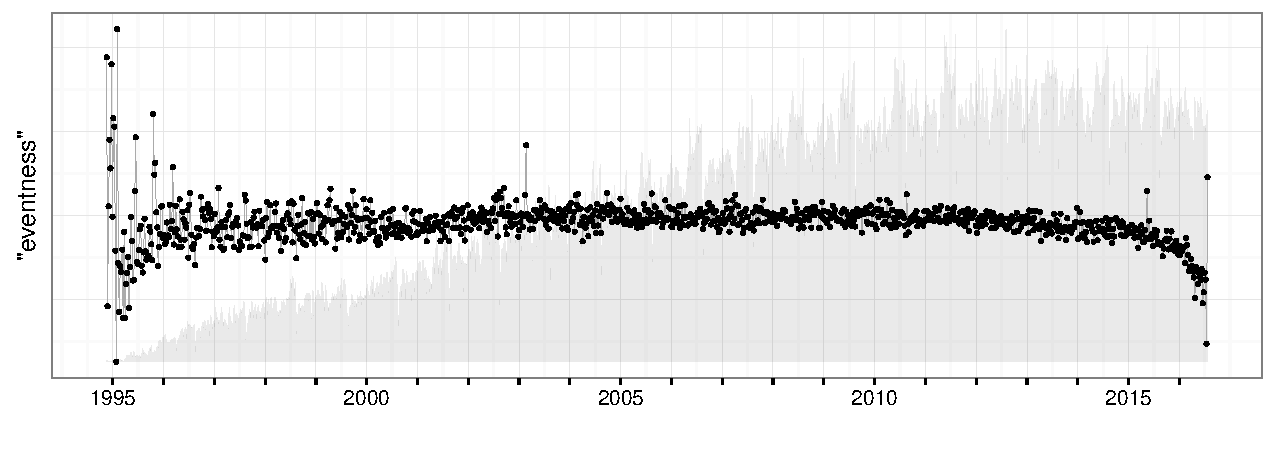
\includegraphics[width=\linewidth]{fig/arxiv_events.pdf}
\caption{Measure of ``eventness'' over arXiv content, \Cref{eq:eventness}.  Grey background indicates the number of abstracts submitted over time.}
\label{fig:arxiv_events}
\end{figure*}

\parhead{Model Sensitivity.}  Using simulated data, we assessed the sensitivity of our model to different decay functions $f$ and decay durations $\tau$.  We simulated data following the description in \Cref{sec:eval}.  We considered an exponential decay function, shown in \Cref{eq:f}, as well as linear decay,
\begin{equation}
f(i_d, t) = 
\begin{cases}
    1 - \frac{i_d - t}{\tau + 1},			& \text{if } t \le i_d < t+\tau  \\
    0,          & \text{otherwise.}
\end{cases}
\label{eq:flinear}
\end{equation}
and a step function,
\begin{equation}
f(i_d, t) = 
\begin{cases}
    1,			& \text{if } t \le i_d \le t+\tau  \\
    0,          & \text{otherwise.}
\end{cases}
\label{eq:fstep}
\end{equation}
We simulated data with $\tau=3$ and simulated ten data sets for each of the three functions $f$.

In fitting the models, we also considered all three functions $f$, but we also varied the decay duration $\tau$ from 1 to 5.  \Cref{fig:sensitivity} shows the results of these experiments, using both event detection and document recovery metrics discussed in \Cref{sec:eval}.

\begin{figure*}[th]
\centering
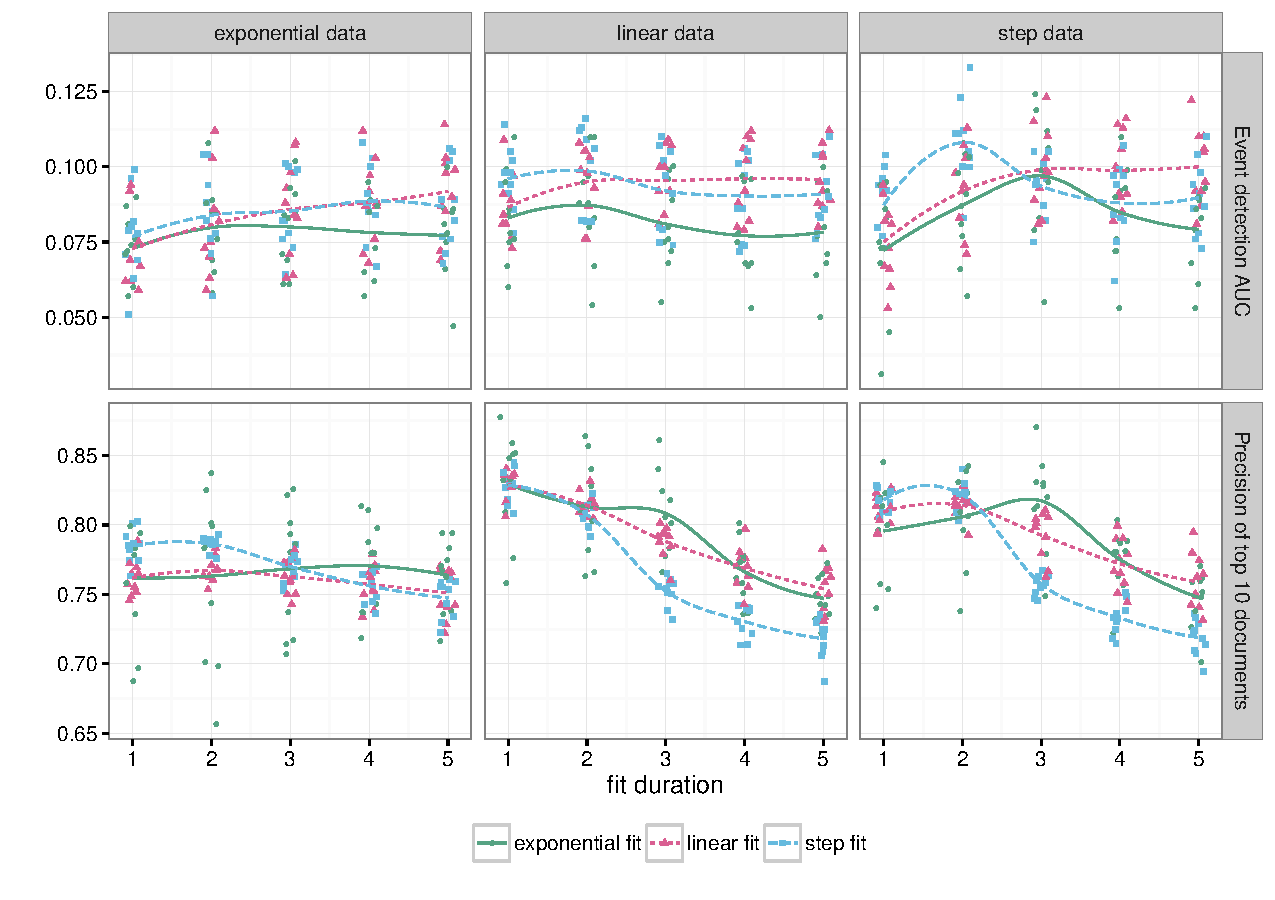
\includegraphics[width=\linewidth]{fig/sim_sensitivity.pdf}
\caption{Assessment of model parameter sensitivity on simulated data--exponential decay tends to perform the best for document recovery, but by a small margin.}
\label{fig:sensitivity}
\end{figure*}

For event detection, the various decay functions perform roughly comparably.  For document recovery, the exponential function has mild advantages on all data types.  In exploring results on the real-world cable data, we found that the exponential decay provided the mos interpretable results.




% We assessed the sensitivity of our model to three different decay functions $f$: exponential, linear, and step functions.  We simulated data for each function and then fit Capsule using every permutation of $f$ and multiple settings for event decay duration.  In all cases, we found that the model is not sensitive to decay shape or duration; details are in Appendix~\ref{sec:additional_results}.

%TODO:
% go through and check citation styles [ ~\cite{Gusfield:97} and Gusfield~\shortcite{Gusfield:97} ]


% \section*{Acknowledgments}

% Do not number the acknowledgment section. %TODO

\bibliography{library.bib}
\bibliographystyle{emnlp2016}

\end{document}
